\section{Model2DPoint  Class Reference}
\label{class_Model2DPoint}\index{Model2DPoint@{Model2DPoint}}
A point robot in a 2D world. 


{\tt \#include $<$model2d.h$>$}

Inheritance diagram for Model2DPoint::\begin{figure}[H]
\begin{center}
\leavevmode
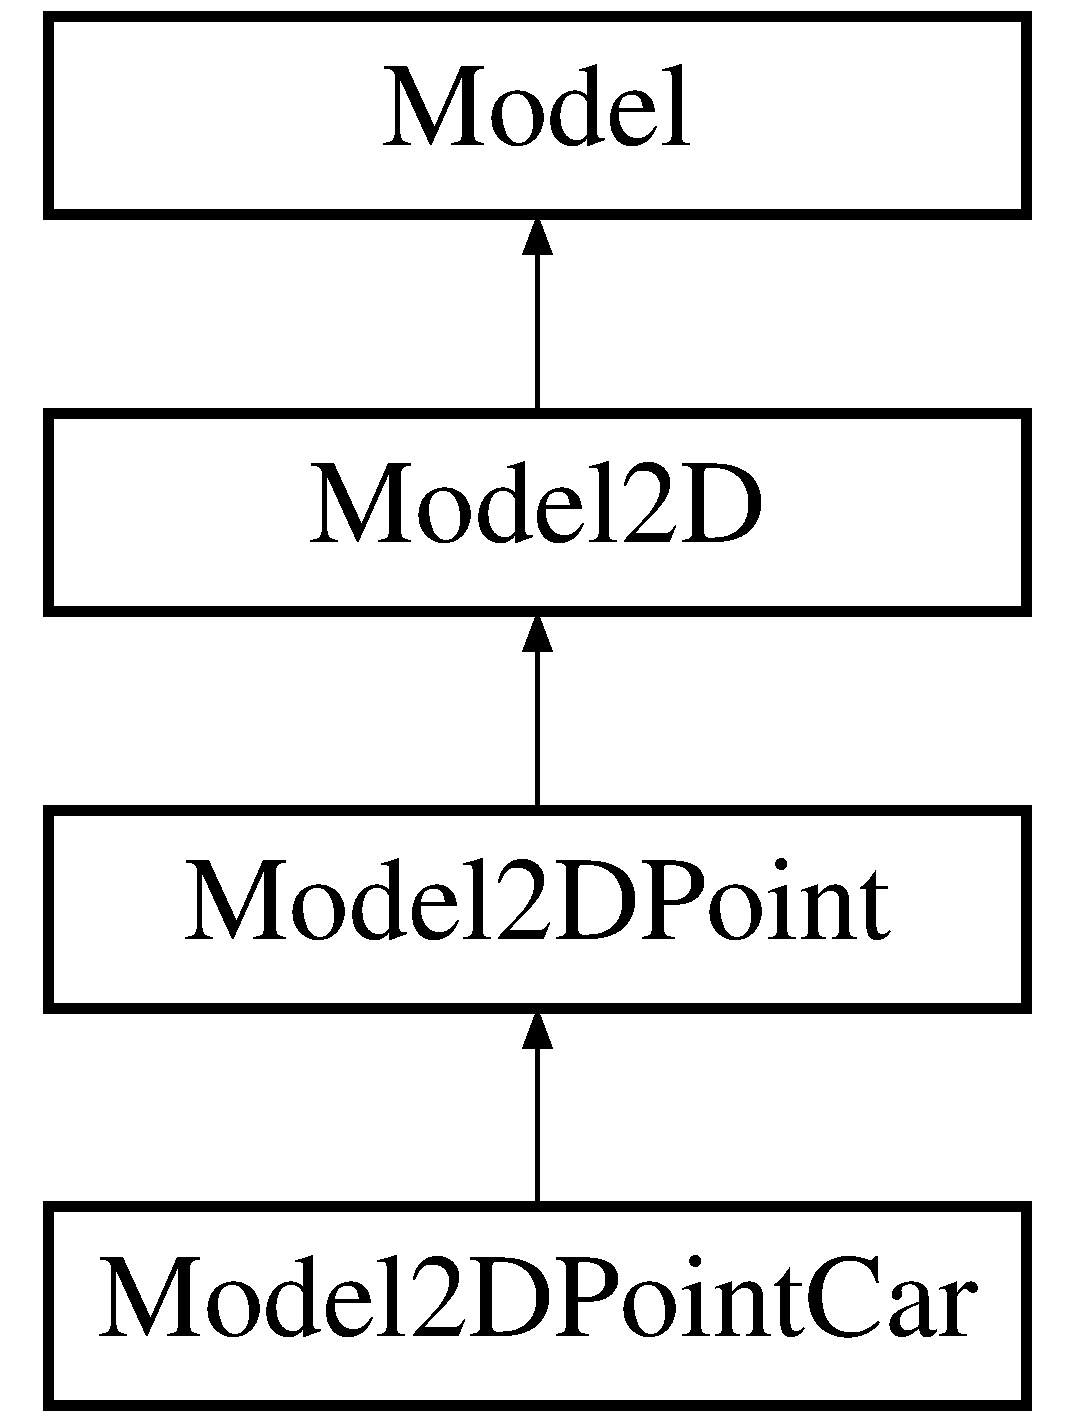
\includegraphics[height=4cm]{class_Model2DPoint}
\end{center}
\end{figure}
\subsection*{Public Methods}
\begin{CompactItemize}
\item 
{\bf Model2DPoint} (string path)
\item 
virtual {\bf $\sim$Model2DPoint} ()
\item 
virtual {\bf MSLVector} {\bf Integrate} (const {\bf MSLVector} \&x, const {\bf MSLVector} \&u, const double \&h)
\begin{CompactList}\small\item\em Perform integration from state x, using input u, over time step h.\item\end{CompactList}\item 
virtual {\bf MSLVector} {\bf State\-Transition\-Equation} (const {\bf MSLVector} \&x, const {\bf MSLVector} \&u)
\begin{CompactList}\small\item\em The state transition equation, or equations of motion, xdot=f(x,u).\item\end{CompactList}\item 
virtual double {\bf Metric} (const {\bf MSLVector} \&x1, const {\bf MSLVector} \&x2)
\begin{CompactList}\small\item\em A distance metric, which is Euclidean in the base class.\item\end{CompactList}\end{CompactItemize}


\subsection{Detailed Description}
A point robot in a 2D world.



\subsection{Constructor \& Destructor Documentation}
\index{Model2DPoint@{Model2DPoint}!Model2DPoint@{Model2DPoint}}
\index{Model2DPoint@{Model2DPoint}!Model2DPoint@{Model2DPoint}}
\subsubsection{\setlength{\rightskip}{0pt plus 5cm}Model2DPoint::Model2DPoint (string {\em path})}\label{class_Model2DPoint_a0}


\index{Model2DPoint@{Model2DPoint}!~Model2DPoint@{$\sim$Model2DPoint}}
\index{~Model2DPoint@{$\sim$Model2DPoint}!Model2DPoint@{Model2DPoint}}
\subsubsection{\setlength{\rightskip}{0pt plus 5cm}Model2DPoint::$\sim$Model2DPoint ()\hspace{0.3cm}{\tt  [inline, virtual]}}\label{class_Model2DPoint_a1}




\subsection{Member Function Documentation}
\index{Model2DPoint@{Model2DPoint}!Integrate@{Integrate}}
\index{Integrate@{Integrate}!Model2DPoint@{Model2DPoint}}
\subsubsection{\setlength{\rightskip}{0pt plus 5cm}virtual {\bf MSLVector} Model2DPoint::Integrate (const {\bf MSLVector} \& {\em x}, const {\bf MSLVector} \& {\em u}, const double \& {\em h})\hspace{0.3cm}{\tt  [virtual]}}\label{class_Model2DPoint_a2}


Perform integration from state x, using input u, over time step h.



Reimplemented from {\bf Model} {\rm (p.\,\pageref{class_Model_a5})}.

Reimplemented in {\bf Model2DPoint\-Car} {\rm (p.\,\pageref{class_Model2DPointCar_a2})}.\index{Model2DPoint@{Model2DPoint}!Metric@{Metric}}
\index{Metric@{Metric}!Model2DPoint@{Model2DPoint}}
\subsubsection{\setlength{\rightskip}{0pt plus 5cm}virtual double Model2DPoint::Metric (const {\bf MSLVector} \& {\em x1}, const {\bf MSLVector} \& {\em x2})\hspace{0.3cm}{\tt  [virtual]}}\label{class_Model2DPoint_a4}


A distance metric, which is Euclidean in the base class.



Reimplemented from {\bf Model} {\rm (p.\,\pageref{class_Model_a9})}.

Reimplemented in {\bf Model2DPoint\-Car} {\rm (p.\,\pageref{class_Model2DPointCar_a4})}.\index{Model2DPoint@{Model2DPoint}!StateTransitionEquation@{StateTransitionEquation}}
\index{StateTransitionEquation@{StateTransitionEquation}!Model2DPoint@{Model2DPoint}}
\subsubsection{\setlength{\rightskip}{0pt plus 5cm}virtual {\bf MSLVector} Model2DPoint::State\-Transition\-Equation (const {\bf MSLVector} \& {\em x}, const {\bf MSLVector} \& {\em u})\hspace{0.3cm}{\tt  [virtual]}}\label{class_Model2DPoint_a3}


The state transition equation, or equations of motion, xdot=f(x,u).



Reimplemented from {\bf Model} {\rm (p.\,\pageref{class_Model_a3})}.

Reimplemented in {\bf Model2DPoint\-Car} {\rm (p.\,\pageref{class_Model2DPointCar_a3})}.

The documentation for this class was generated from the following file:\begin{CompactItemize}
\item 
{\bf model2d.h}\end{CompactItemize}
